%%% Local Variables:
%%% mode: latex
%%% TeX-master: t
%%% End:

\chapter{应用——某嵌入式软件的中断时间性质分析和验证}
\label{cha:case}

受中航工业集团动力控制研究所(无锡)委托,我所在实验室为其验证某嵌入式平台上的中
断驱动程序。其中一项重要的验证需求就是验证中断优先级设置的合理性。换句话说,我们
需要验证中断在既有优先级的设置下,其实时性得到保障。我正是应用第~\ref{cha:intr} 
章描述的方法和模型,针对本项目做了一些修改,最后完成了该验证需求。

\section{Intel 8259}
\label{sec:8259}

构建形式化模型之前,我们首先需要对该平台的中断实现有一个全面详细的了解。

\begin{figure}[H]
	\centering
	
\includegraphics[width=0.9\textwidth]{8259_internal}
	\caption{8259的内部逻辑}
	\label{fig:8259_internal}
\end{figure}

某嵌入式平台采用Intel 8259芯片控制中断。Intel8259是一系列可编程化中断控制器(
PIC:Programmable Interrupt Controller)芯片的总称,当初设计它是为了搭配 8-bit
的Intel 8085以及16-bit的Intel 8086等微处理器来使用。此系列的芯片原本包含 8259、
8259A、和 8259B,但时至今日,许多制造商已制作了相当多与8259兼容的芯片。运作上,
8259是一个多任务器,它会从多个中断源中挑出一个中断信号,并输出。

8259的内部结构如图~\ref{fig:8259_internal} 所示,其内部结构逻辑主要由以下三部
分组成:

\begin{itemize}
	\item 控制逻辑
	\item 中断优先权判优及其屏蔽
	\item 辅助电路
\end{itemize}

\subsection{编程结构}
\label{subsec:8259_program}

8259的编程结构共由10个寄存器构成,每个寄存器均为8位。如图~\ref{fig:8259_program}
所示。

\begin{figure}[H]
	\centering
	
\includegraphics[width=0.9\textwidth]{8259_program}
	\caption{8259的编程结构}
	\label{fig:8259_program}
\end{figure}

10个寄存器可分为三组。第一组:IRR、PR、ISR。

\begin{description}
	\item[IRR] 中断请求寄存器(Interrupt Request Register) 该寄存器的8位(D
	7~D0)分别存放IR7~IR0输入线上的中断请求。当某输入线有请求时,IRR对应位置1,
	该寄存器具有锁存功能。
	\item[ISR] 当前中断服务寄存器(In Service Register) 该寄存器用于存放正在
	被服务的所有中断级,包括尚未服务完而中途被别的中断打断了的中断级。
	\item[PR] 优先级裁决器(Priority Resolver) 当IR输入线上有请求时,IRR对应
	位置1,同时,PR将该中断的优先级与ISR中的优先级比较,若该中断的优先级高于ISR
	中的最高优先级,则PR就使INT信号变为高电平,把该中断送给CPU,同时,在ISR相应
	位置1。否则,PR不为该中断提出申请。
\end{description}

第二组:ICW1、ICW2、ICW3、ICW4。这四个寄存器用来存放初始化命令字(Initialization 
Command Word)。初始化命令字一般在系统启动时由程序设置,一旦设定,一般在系统工作
过程中就不再改变。

\begin{description}
	\item[ICW1] 指定本8259是否与其他8259级联,以及中断请求输入信号的形式(边沿
	触发/电平触发)。
	\item[ICW2] 指定中断类型码。
	\item[ICW3] 指定本8259与其他8259的连接关系。
	\item[ICW4] 指定本片8259的中断结束方式、中断嵌套方式、与数据总线的连接方式
	(缓冲/非缓冲)。
\end{description}

第三组:OCW1、OCW2、OCW3。这三个寄存器用于存放操作命令字(Operation Command 
Word)。操作命令字由应用程序使用,以便对中断处理过程作动态控制。在系统运行过程中,
操作命令字可以被多次设置。

\begin{description}
	\item[OCW1] 又称中断屏蔽寄存器(IMR:Interrupt Mask register),当其某位置
	1时,对应的IR线上的请求被屏蔽。例如,若OCW1的D3位置1,当IR3线上出现请求时,
	IRR的D3位置1,但8259不把IR3的请求提交优先级仲裁器PR裁决,从而,该请求没有机
	会被提交给CPU。
	\item[OCW2] 指定优先级循环方式及中断结束方式。
	\item[OCW3] 指定8259内部寄存器的读出方式、设定中断查询方式、设定和撤消特殊
	屏蔽方式。
\end{description}

\subsection{功能}
\label{subsec:8259_function}

8259通过以下4个功能来完成中断管理器的工作。

\begin{enumerate}[(1)]
	\item 一片Intel 8259可管理8个中断请求,并把当前优先级最高的中断请求送到CPU
	的INTR端。
	\item 当CPU响应中断时,为CPU提供中断类型码。
	\item 8个外部中断的优先级排列方式,可以通过对8259编程进行指定。也可以通过编
	程屏蔽某些中断请求,或者通过编程改变中断类型码。
	\item 允许9片8259级联,构成64级中断系统。在微机中,使用两片8259级联,构成15
	级中断,其连接情况如图~所示。
\end{enumerate}

\begin{figure}[H]
	\centering
	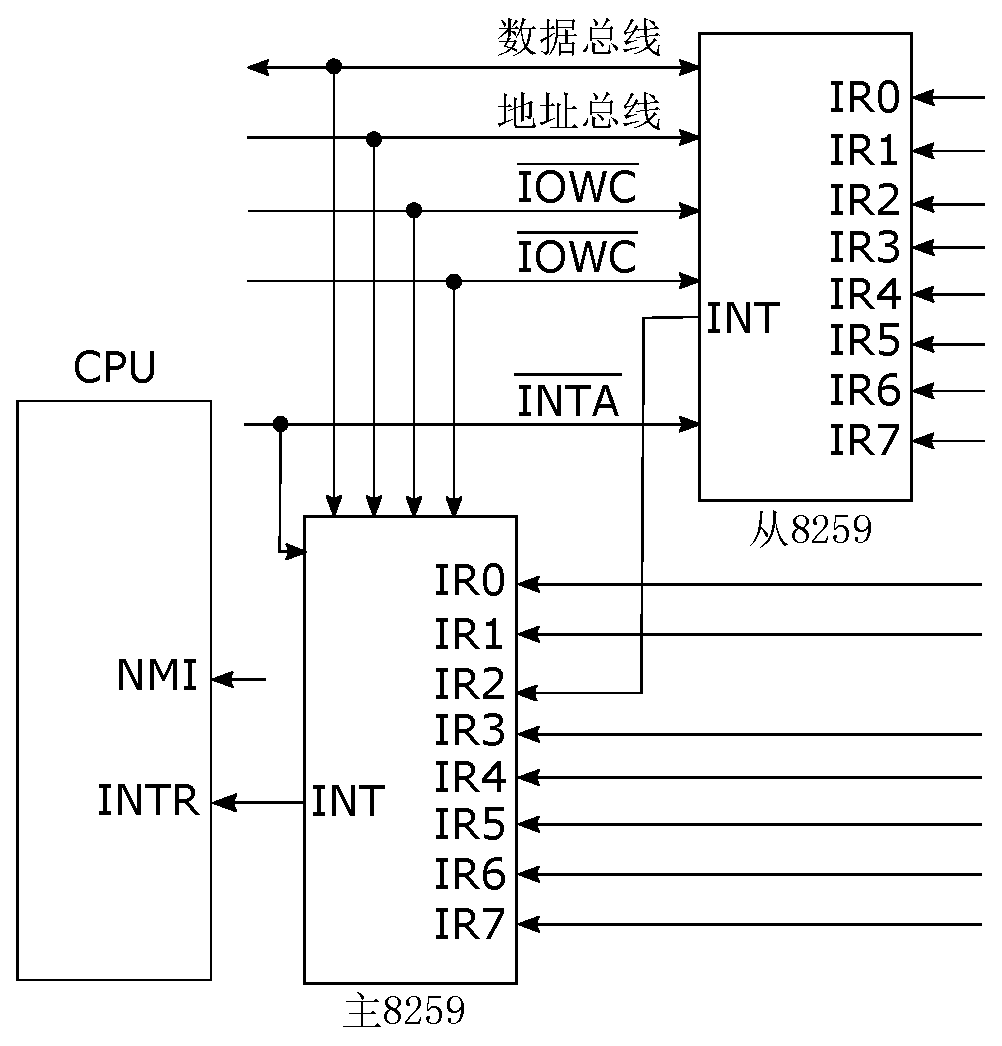
\includegraphics[width=0.6\textwidth]{8259_cascad}
	\caption{8259的编程结构}
	\label{fig:8259_cascad}
\end{figure}

\subsection{工作原理}
\label{subsec:8259_work}

8259完成一次中断处理的工作步骤如下:

\begin{enumerate}[(1)]
	\item 线上提出了中断请求的中断源,即出现请求,IRR中断请求寄存器(共有8位D7~
	D0)对应于连接在IR0~IR7线上的外设的中断请求,哪一根输入线有请求,哪一根输入
	线就置1。。
	\item 若OCW1(IMR中断屏蔽寄存器)未使该中断请求屏蔽(对应位为0时不屏蔽),
	该请求被送入PR(优先权分析器)比较。否则,不送入PR比较。	
	\item 把新进入的请求与ISR(服务中寄存器)中正在被处理的中断进行比较。如果新
	进入的请求优先级较低,则8259不向CPU提出请求。如果新进入的请求优先级较高,则
	8259使INT引脚输出高电平,向CPU提出请求。
	\item 如果CPU内部的标志寄存器中的IF(中断允许标志)为0,CPU不响应该请求。若
	IF=1,CPU在执行完当前指令后,从CPU的INTA引脚上向8259发出两个负脉冲。
	\item 第一个 INTA负脉冲到达8259时,8259完成以下三项工作:
	\begin{enumerate}[a.]
		\item 使IRR的锁存功能失效。这样一来,在IR7~IR0上的请求信号就不会被8259
		接收。直到第二个INTA负脉冲到达8259时,才又使IRR的锁存功能有效。 
		\item 使ISR中的相应位置1。
		\item 使IRR中的相应位清0。
	\end{enumerate}
	\item 第二个INTA负脉冲到达8259时,8259完成以下工作:
	\begin{enumerate}[a.]
		\item 将中断类型码(ICW2中的值)送到数据总线上,CPU将其保存在“内部暂存器”
		中。
		\item 如果ICW4中设置了中断自动结束方式,则将ISR的相应位清0。
	\end{enumerate}
	\item CPU把PSW(程序状态控制字)入栈。
	\item PSW中的IF、TF清0。
	\item CS入栈。
	\item IP入栈。
	\item 根据内部暂存器的值获得中断向量表中的位置,从中断向量表内取出一字,送
	CS。
	\item 从中断向量表内取出一字,送IP。
	\item 至此,CPU转入中断处理程序执行。在中断处理程序中,IF为0,CPU不会响应
	新的8259的请求。(同时,TF=0,不允许单步执行中断处理程序)。但在中断处理程
	序中,可以使用STI指令(开中断,使IF=1),使CPU允许响应新的8259的请求,这样
	一来,如果8259有更高优先级的请求,该中断处理程序将被中断,出现了中断嵌套。
	\item 中断处理程序的最后一条指令为IRET(中断返回)。该指令从堆栈中取出(8)
	\pozhehao (10)步保存的IP、CS、PSW,CPU接着执行被中断的程序。
\end{enumerate}

\section{中断设置}
\label{sec:intr_setting}

某嵌入式平台采用两片Intel 8259级联的方式,如图3所示。我们称与CPU连接的Intel 8259
为主片,与主片连接的另一片为从片。该项目中涉及中断共10个,主从片上各5个。通过设置
主片上的OCW2寄存器,使主片上中断优先级为IR3$>$IR4$>$IR5$>$IR6$>$IR7$>$IR0$>$IR1
$>$IR2。因为IR2上连接的是从片,因此主片上中断优先级比从片高。从片上中断优先级按默
认设置,IR0$>$IR1$>$IR2$>$IR3$>$IR4$>$IR5$>$IR6$>$IR7。主从片上中断优先级固定,
没有动态变化。同时,因为需要保持从片上高优先级中断可以抢占低优先级中断这一性质,主
片上的IR2需要可以打断自身,因此通过设置主片上ICW4寄存器使主片上中断能够被自身打断。
从片上中断均不可打断自身。

10个中断中,有3个通讯中断在实际运行中不会被触发。因此我们需要考虑的中断数量是7个。

\section{\uppaal 简介}
\label{sec:Uppaal_intro}

\uppaal 是一个进行建模,仿真和验证实时系统的集成工具环境,由丹麦奥尔堡大
学的计算机科学基础研究中心(Basic Research in Computer Science, BRICS)
和瑞典乌普萨拉大学信息技术系联合开发。它适合那些可以被建模为具有有限的控
制结构和实数值时钟,通过信道或共享变量通信的非确定性过程集合的系统。典型
的应用领域包括实时控制器和特定的实时性至关重要的通信协议。\cite{Behrmann04atutorial}

\section{在\uppaal 中构建中断模型}
\label{sec:build}

在与对方工程师交流之后,我们认为一个中断在处理结束之前,它的下一个实例触发,会对
数据造成不可预计的影响。中断优先级的设置目的则是避免该情况的发生。于是,问题转换
为如何验证中断能否在它的下一个实例触发之前被处理完。这个性质在自动机模型里表达起
来却是有一定的难度,因为我们并不能准确预知某中断的下一个实例何时触发。幸运的是,
在本项目中,我们有足够的信息来确定某中断触发后,下一个实例最早可能什么时候触发。
即,如果中断能在该时刻到来前处理完成,就满足实时性需求。

\begin{definition}
	$T^\prime$表示允许的中断响应耗时的上限。
	\label{def:T_prime}
\end{definition}

对于定时中断,我们只需要将中断流逝时间设置为定时周期即可。对于其他中断,我们可以
根据实际运行场景给出一个合理的流逝时间上限。非定时中断分为两类。一类是通讯中断。
受通讯线路的物理特性限制,一个通讯中断两次触发之间有一个最小的时间间隔。该时间间
隔有通讯传输的比特率和每次中断处理的数据量共同决定,因此可以计算出来。我们将这个
时间间隔作为通讯中断的流逝时间上限。另一类是AD中断,该中断有程序中特定位置启动一
次AD转换,在转换完成之后触发。每5ms为一个周期,AD中断会被连续触发5-6次。为简化模
型,我们引入一个假设。

\begin{assumption}
	同一个5ms周期内的AD中断的处理时间没有重叠且在上一个AD中断实例执行结束以后下
	一个AD中断实例马上触发。
	\label{assume:ad}
\end{assumption}

在假设~\ref{assume:ad} 的约束下,我们可以将一个5ms周期中的6次AD中断合并为一个。
取6次而不是5次,则是为了验证的完备性。如果6次AD中断都不会超时,5次AD中断自然也
不会。简化以后,每个5ms周期会有一个AD中断,因此我们把AD中断的流逝时间上线设置为
5ms。

在上述分析之后,我们构建中断模型时即不需要表现出中断可重入这一性质。因为如果发生
中断重入,即上一个中断实例没能在流逝时间上限内运行完成。这种情况我们认为是一个错
误,因此一旦发生,模型运行即可停止。我们建立的模型的运行是不需要中断重入这一行为。
所有中断均可用一个状态机来描述。AD中断,由于在中断处理函数里有EOI的操作,会将ISR
对应位置0,行为特殊,用一个状态机来单独描述。除此以外,我们需要一个中断源,它会
按照一定的条件约束触发中断。该中断源也用一个状态机来描述。

%//    0 SIO0
%//    1 双发通讯
%//    2 AD        分割为两部分,第二部分的优先级为10,可被任意中断打断
%//    3 Timer1, 小闭环    从该中断开始,每个中断都能被自身打断
%//    4 Timer2,大闭环
%//    5 DMA结束
%//    6 DMA应答

\subsection{声明}
\label{subsec:exp_decl}

该模型的声明比较长,分列在图~\ref{fig:exp_decl} 和图~\ref{fig:exp_decl_2} 中。

\begin{figure}[H]
	\centering
	\begin{lstlisting}
	const int N = 7;
	typedef int[0, N-1] intr_id; 	
	const int minInterval_0 = 50; //0号中断最短间隔
	const int minInterval_1 = 50; //1号中断最短间隔	
	//3号中断运行了120us,第一个AD可以触发
	const int AD_start = 120; 	
	chan intr[intr_id];
	urgent broadcast chan prompt, resume;	
	// 中断响应耗时上限
	const int D[intr_id] = {minInterval_0, minInterval_1, 
							500, 500, 2500, 2500, 2500};
	// 中断执行所需时间 
	const int E[intr_id] = {1, 1, 2, 125, 1011, 6, 8}; 
	const int cTime = 2; // AD无中断特权部分执行的时间, 16us
	bool IRR[intr_id] = {false, false,false,false,
						false,false,false};
	bool ISR[intr_id] = {false, false,false,false,
						false,false,false};
	int ICG[intr_id] = {50, 2, 5, 5, 1, 1, 1}; 
	int fix_count[intr_id] = {0, 0, 0, 0, 0, 0, 0};
	int fix_count_non;	
	intr_id stack[N+1]; // 中断栈
	typedef int[0,N] SP;
	SP sp = 0; // 栈顶指针
	clock intTime[intr_id];
	clock timeSinceStart[intr_id];
	clock universe;	
	\end{lstlisting}
	\caption{某嵌入式平台中断模型:声明}
	\label{fig:exp_decl}
\end{figure}

\begin{figure}[H]
	\centering
	\begin{lstlisting}[firstnumber=28]
	bool already[intr_id] = {false, false, false, false, 
							false, false, false};	

	typedef int[0,N] Pri;
	Pri get_highest_pri(){
		meta int i;
		for(i = 0; i < N; i++){
			if(ISR[i] || IRR[i]){
				return i;
			} 
		}
		return N;
	}
	
	int get_highest_irr(){
		meta int j;
		for(j = 0; j < N; j++){
			if(IRR[j]){
				return j;
			} 
		}
		return N;
	}
	
	int get_highest_isr(){
		meta int k;
		for(k = 0; k < N; k++){
			if(ISR[k]){
				return k;
			} 
		}
		return N;
	}
	
	int fix_time(){
		meta int i;
		int t = 0;
		for(i = 0; i < N; i++){
			t = t + fix_count[i] * E[i];
		}
		t = t + fix_count_non * cTime;
		return t;
	} 
	\end{lstlisting}
	\caption{续:某嵌入式平台中断模型:声明}
	\label{fig:exp_decl_2}
\end{figure}

其中部分定义与~\ref{subsubsec:basic_decl} 小节中类似。在第1行,我们定义了
中断数目,第2行依然是重新定义一个数据类型用来表示中断ID和优先级。第3、4行分
别定义了0号和1号中断\footnote{由于项目涉密,在此提到的所有的具体中断名均省
略,以中断ID代替。AD中断为2号中断。}的触发最短时间间隔。第6行定义了一个时间
间隔,在~\ref{subsec:exp_env} 小节中我们在定义中断触发源时会使用它。之所以
将数值定义在这里是为了集中所有静态定义,方便修改和实验调整。

第7、8行定了所有的信道。第10-14定义了所有的时间参数的数值,E[]和D[]分别存储
$T$和$T^\prime$的数值。其中cTime是AD中断的无中断特权部分的执行时间,关于AD
中断我们将在\ref{subsec:exp_ad} 小节详细介绍。第19行定义了每个中断的发生次
数。因为需要验证的程序的中断具有周期性,因此我们只需要验证一个最大周期内的情
况即可。而一个最大周期内各个中断的触发次数是已知的。

第20、21行和62-70行定义的是修正估计时间相关的数据和函数。这是由于\uppaal 在
估算时间的时候区间不够准确,因此我们引入了一个修正。第22行定义了一个数组来
模拟栈。这个栈内不是具体的数据,而是某个中断触发了。在之前的建模中我们都不
需要栈,是因为一直都没有出现过优先级反转的情况,我们只需要有ISR寄存器就能判
断接下来该哪一个中断执行。然而,在本例中,由于AD中断的特殊设置,出现了优先
级反转,因此在建模时,我们不得不引入栈来保证中断语义的正确性。

第25-27行定义了所有的时钟,之所以定义在这里而不放在模板内部,是因为中断触发
源需要部分读取时钟。放在声明里与放在模板内部对状态空间的大小并没有影响。

第28行定义了一个数组来表示某中断在本周期是否已经触发过。这个数组是为了表达
中断先后触发的语义设置的,详细的使用见\ref{subsec:exp_model_decl} 小节。

第31-60行顶一个几个辅助函数。代码逻辑都很简单,在此不赘述。

\subsection{普通中断模板}
\label{subsec:exp_intr}

本项目中,普通中断的状态机如图~\ref{fig:exp_decl} 所示。它的构造很简单,
和~\ref{subsubsec:basic_decl} 小节中展示的状态机类似,但是有三个主要区别:

\begin{itemize}
	\item 本状态机有一个Error位置。设置该位置是为了便于描述验证性质。
	\item 部分参数和内部声明省略,直接使用声明中的定义。
	\item 没有忽略本中断的其他实例。这是因为在抽象过程中我们已经保证正确
	运行的时候,不会有本中断的下一个实例在当前实例完成之前到来。
\end{itemize}

模板只有一个参数\pozhehao 中断ID,没有内部声明,位置和变迁说明见
表~\ref{tab:exp_intr_loc} 和~\ref{tab:exp_intr_mov} 。

\begin{figure}[H]
	\centering
	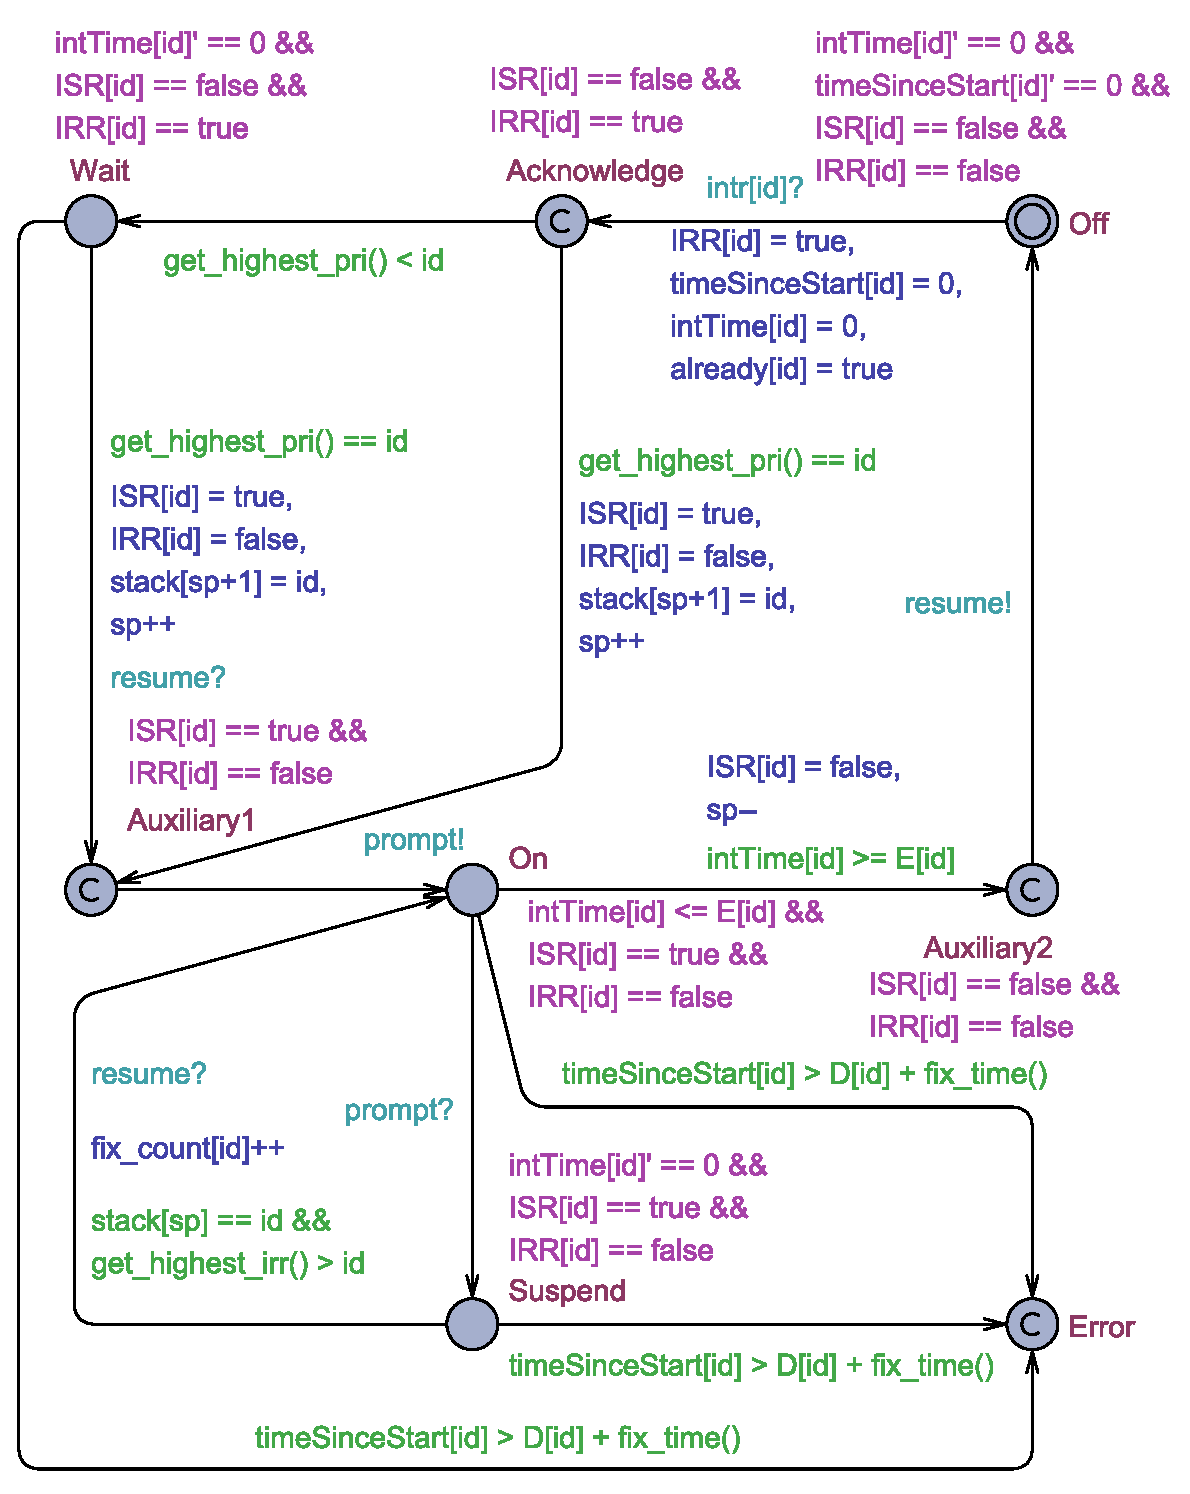
\includegraphics[width=0.9\textwidth]{Interrupt}
	\caption{某嵌入式平台中断模型:普通中断}
	\label{fig:exp_intr}
\end{figure}

\begin{longtabu} to \linewidth {p{5em}p{5em}p{13em}X}
	\caption{某嵌入式平台中断模板:位置}
	\label{tab:exp_intr_loc}\\
	\toprule[1.5pt]
	{\heiti 名称} & {\heiti 附加属性} & {\heiti 约束} & {\heiti 含义}\\
	\midrule[1pt]
	\endfirsthead
	\multicolumn{4}{c}{续表~\thetable\hskip1em 基本中断模板:位置}\\
	\toprule[1.5pt]
	{\heiti 名称} & {\heiti 附加属性} & {\heiti 约束} & {\heiti 含义}\\
	\midrule[1pt]
	\endhead
	\hline
	\multicolumn{4}{r}{续下页}
	\endfoot
	\endlastfoot
	Off & 初始位置 & intTime和timeSinceStart保持静止,ISR和IRR对应位为false & 
	初始位置,当前没有该中断\\
	\midrule[0.5pt]
	Acknowledge & 关键位置 & ISR对应位为false,IRR对应位为true & 中断控制器
	接收到中断信号\\
	\midrule[0.5pt]
	Wait & & intTime保持静止,ISR对应位为false, IRR对应位为true & 当前有优先
	级更高的中断在运行,本中断等待。\\
	\midrule[0.5pt]
	Auxiliary1 & 关键位置 & ISR对应位为true,IRR对应位为false & 为表达Wait和
	Acknowledge到On的语义设置的辅助位置\\
	\midrule[0.5pt]
	On & & intTime不超过E[id](中断处理时间$T$),ISR对应位为true,IRR对
	应位为false & 中断正在被处理 \\
	\midrule[0.5pt]
	Suspend & & intTime静止,ISR对应位为true,IRR对应位为false & 中断被更高
	优先级的中断抢占CPU \\ 
	\midrule[0.5pt]
	Auxiliary2 & 关键位置 & ISR对应位为false,IRR对应位为false & 为表达On到
	Off的完整语义设置的辅助位置\\
	\midrule[0.5pt]
	Error & 关键位置 &  & 中断未在中断响应时间上限之内完成\\
	\bottomrule[1.5pt]
\end{longtabu}

\begin{longtabu} to \linewidth {p{5em}p{5em}XXXX}
	\caption{嵌入式平台中断模板:变迁 }
	\label{tab:exp_intr_mov}\\
	\toprule[1.5pt]
	{\heiti 迁出位置} & {\heiti 迁入位置} & {\heiti 条件} & {\heiti 同步} & 
	{\heiti 更新} & {\heiti 含义}\\
	\midrule[1pt]
	\endfirsthead
	\multicolumn{6}{c}{续表~\thetable\hskip1em 基本中断模板:变迁}\\
	\toprule[1.5pt]
	{\heiti 迁出位置} & {\heiti 迁入位置} & {\heiti 条件} & {\heiti 同步} & 
	{\heiti 更新} & {\heiti 含义}\\
	\midrule[1pt]
	\endhead
	\hline
	\multicolumn{6}{r}{续下页}
	\endfoot
	\endlastfoot
	Off & Acknowledge & & 接收到中断信号 & IRR对应位置位,时钟清零 & 中断控
	制器接收到中断信号\\
	\midrule[0.5pt]
	Acknowledge & Wait & 本中断优先级不是最高 & & & 当前有更高优先级的中断存
	在,本中断等待\\
	\midrule[0.5pt]
	Wait & Auxiliary1 & 本中断优先级最高 & 接收到resume信号 & IRR对应位复位,
	ISR对应位置位,本中断入栈 &  高优先级的中断执行完毕,本中断得到CPU\\
	\midrule[0.5pt]
	Acknowledge & Auxiliary1 & 本中断优先级最高 & & IRR对应位复位,ISR对应位
	置位,本中断入栈 & 本中断优先级最高,准备执行\\
	\midrule[0.5pt]
	Auxiliary1 & On & & 发送prompt信号 & & 当前中断获得CPU,打断其他正在被处
	理的中断\\
	\midrule[0.5pt]
	On & Suspend & & 接收到prompt信号 & & 当前中断被更高优先级的中断打断\\
	\midrule[0.5pt]
	Suspend & On & 本中断在栈顶且无更高优先级的中断处在Wait位置 & 接收到resume
	信号 & fix\_count增加 & 高优先级的中断执行完毕,本中断得到CPU\\
	\midrule[0.5pt]
	On & Auxiliary2 & intTime[id]达到E[id] & & ISR对应位复位,本中断出栈 & 
	中断执行结束\\
	\midrule[0.5pt]
	Auxiliary2 & Off & & 发送resume信号 & & 通知其他中断获取CPU\\
	\midrule[0.5pt]
	Wait & Error & 中断响应时间超过上限 & & & 中断处理超时\\
	\midrule[0.5pt]
	On & Error & 中断响应时间超过上限 & & & 中断处理超时\\
	\midrule[0.5pt]
	Suspend & Error & 中断响应时间超过上限 & & & 中断处理超时\\
	\bottomrule[1.5pt]
\end{longtabu}

注意在Auxiliary2到Off的变迁中,时钟没有清零。这是因为在~\ref{subsec:exp_env} 
小节中的中断源需要用到intTime[id]时钟里的数据来表达中断触发的时序关系。

\subsection{AD中断模板}
\label{subsec:exp_ad}

AD中断是一个特殊的中断。它与~\ref{subsubsec:segment_intr} 小节中提到的分段中断
类似,也是一个分段中断。然而它的分段的实现并非依赖一个类似于eCos那样完整的机制,
而是在中断自身调用特殊指令EOI清除了中断服务位,即将ISR寄存器对应位复位。这样做并
不会立即跳转其他中断去执行,之前被AD中断抢占的的其他中断依旧被抢占着。但是之后触
发的任何中断都会打断AD中断,抢占CPU。如果后来的中断优先级较低,那么就会造成优先
级反转。另外,在后来的中断运行结束之后,CPU会回到AD中断执行。尽管此时看ISR寄存器
的话,AD中断的对应位为0而有其他中断的对应位为1。因为恢复现场是按照退栈的顺序进行
的,这也是为什么我们在该模型中不得不引入一个栈。

除此以外,抽象时,我们将一个小周期内的连续6个AD中断看成了一个以减小状态空间,那
么一个AD中断内部的变迁就需要变得复杂一些。由于原本每个AD中断被分成了两部分,在模
型中的AD中断就会被分成$2\times 6$段。

AD中断的状态机如图~\ref{fig:exp_AD} 所示。AD的参数只有中断ID,内部声明只有一个
用来计数的count。AD中断的位置和变迁说明分别见表~\ref{tab:exp_AD_loc} 和
表~\ref{tab:exp_AD_mov} 。

\begin{figure}[H]
	\centering
	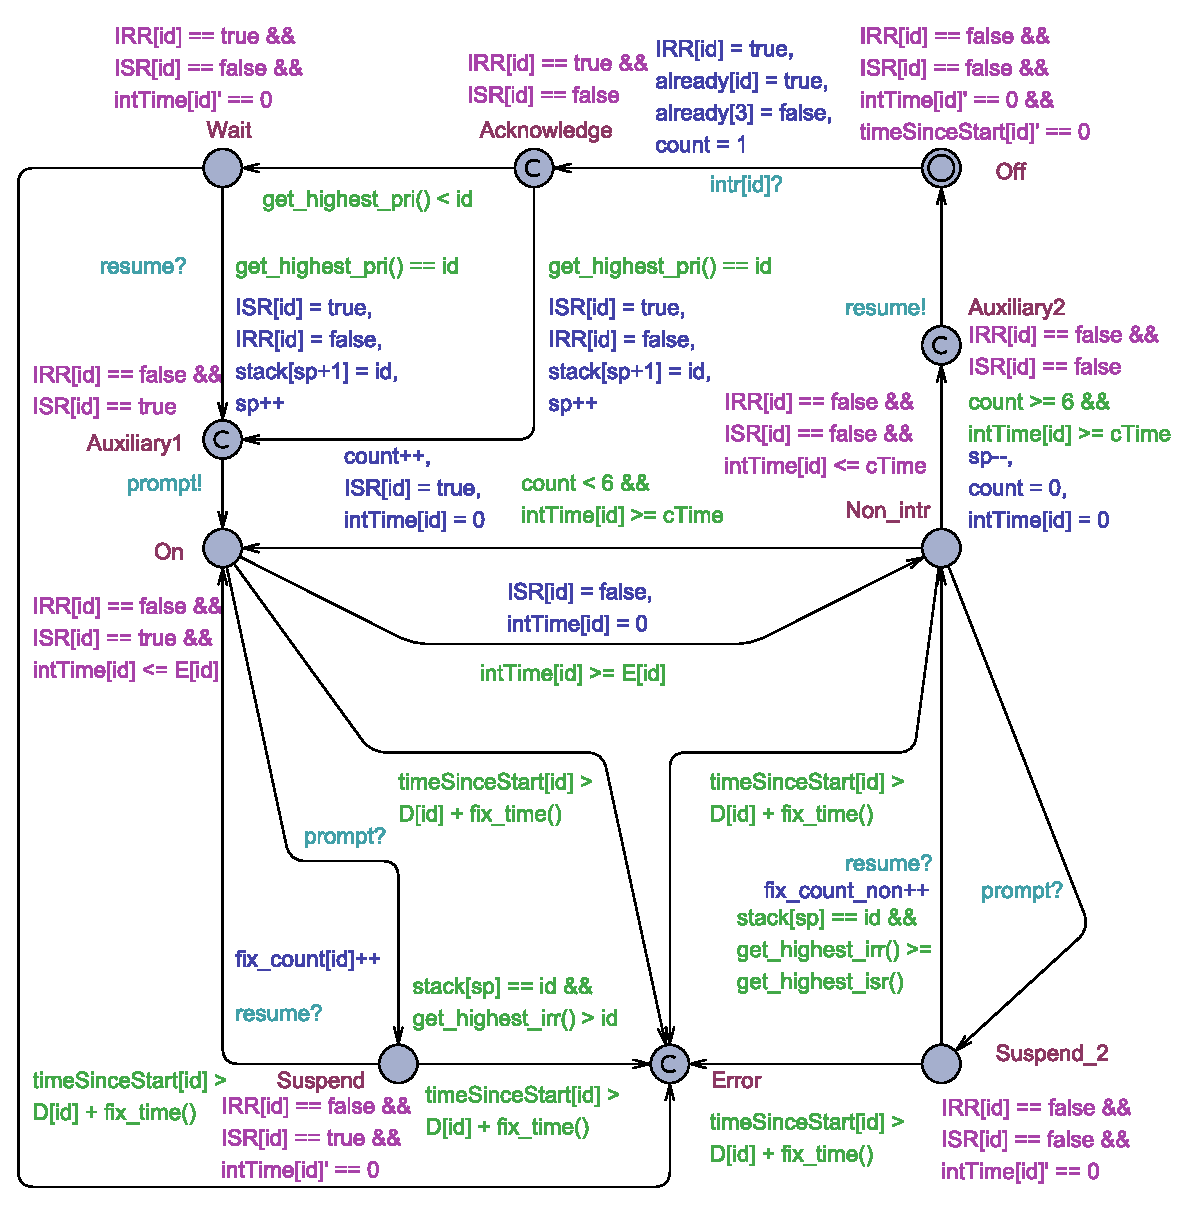
\includegraphics[width=\textwidth]{AD}
	\caption{某嵌入式平台中断模型:AD中断}
	\label{fig:exp_AD}
\end{figure}

\begin{longtabu} to \linewidth {p{5em}p{5em}p{13em}X}
	\caption{某嵌入式平台中断模板:位置}
	\label{tab:exp_AD_loc}\\
	\toprule[1.5pt]
	{\heiti 名称} & {\heiti 附加属性} & {\heiti 约束} & {\heiti 含义}\\
	\midrule[1pt]
	\endfirsthead
	\multicolumn{4}{c}{续表~\thetable\hskip1em 基本中断模板:位置}\\
	\toprule[1.5pt]
	{\heiti 名称} & {\heiti 附加属性} & {\heiti 约束} & {\heiti 含义}\\
	\midrule[1pt]
	\endhead
	\hline
	\multicolumn{4}{r}{续下页}
	\endfoot
	\endlastfoot
	Off & 初始位置 & intTime和timeSinceStart保持静止,ISR和IRR对应位为false & 
	初始位置,当前没有该中断\\
	\midrule[0.5pt]
	Acknowledge & 关键位置 & ISR对应位为false,IRR对应位为true & 中断控制器
	接收到中断信号\\
	\midrule[0.5pt]
	Wait & & intTime保持静止,ISR对应位为false, IRR对应位为true & 当前有优先
	级更高的中断在运行,本中断等待。\\
	\midrule[0.5pt]
	Auxiliary1 & 关键位置 & ISR对应位为true,IRR对应位为false & 为表达Wait和
	Acknowledge到On的语义设置的辅助位置\\
	\midrule[0.5pt]
	On & & intTime不超过E[id](EOI之前的中断处理时间$T_{before}$),ISR对应位
	为true,IRR对应位为false & EOI之前,中断正在被处理\\
	\midrule[0.5pt]
	Suspend & & intTime静止,ISR对应位为true,IRR对应位为false & EOI之前,中
	断被更高优先级的中断抢占CPU \\ 
	\midrule[0.5pt]
	Non\_intr & & intTime不超过cTime(EOI之后的中断处理时间$T_{after}$),
	ISR对应位为false,IRR对应位为false & EOI之后,中断正在被处理\\
	\midrule[0.5pt]
	Suspend\_2 & & intTime静止,ISR对应位为false,IRR对应位为false & EOI之
	后,中断被其他中断抢占CPU \\
	\midrule[0.5pt]
	Auxiliary2 & 关键位置 & ISR对应位为false,IRR对应位为false & 为表达Non\_intr
	到Off的完整语义设置的辅助位置\\
	\midrule[0.5pt] 
	Error & 关键位置 &  & 中断未在中断响应时间上限之内完成\\
	\bottomrule[1.5pt]
\end{longtabu}

\begin{longtabu} to \linewidth {p{5em}p{5em}XXXX}
	\caption{嵌入式平台中断模板:变迁 }
	\label{tab:exp_AD_mov}\\
	\toprule[1.5pt]
	{\heiti 迁出位置} & {\heiti 迁入位置} & {\heiti 条件} & {\heiti 同步} & 
	{\heiti 更新} & {\heiti 含义}\\
	\midrule[1pt]
	\endfirsthead
	\multicolumn{6}{c}{续表~\thetable\hskip1em 基本中断模板:变迁}\\
	\toprule[1.5pt]
	{\heiti 迁出位置} & {\heiti 迁入位置} & {\heiti 条件} & {\heiti 同步} & 
	{\heiti 更新} & {\heiti 含义}\\
	\midrule[1pt]
	\endhead
	\hline
	\multicolumn{6}{r}{续下页}
	\endfoot
	\endlastfoot
	Off & Acknowledge & & 接收到中断信号 & IRR对应位置位,时钟清零,计数器启
	动 & 中断控制器接收到中断信号\\
	\midrule[0.5pt]
	Acknowledge & Wait & AD中断优先级不是最高 & & & 当前有更高优先级的中断存
	在,AD中断等待\\
	\midrule[0.5pt]
	Wait & Auxiliary1 & AD中断优先级最高 & 接收到resume信号 & IRR对应位复位,
	ISR对应位置位,AD中断入栈 &  高优先级的中断执行完毕,AD中断得到CPU\\
	\midrule[0.5pt]
	Acknowledge & Auxiliary1 & AD中断优先级最高 & & IRR对应位复位,ISR对应位
	置位,AD中断入栈 & AD中断优先级最高,准备执行\\
	\midrule[0.5pt]
	Auxiliary1 & On & & 发送prompt信号 & & AD中断获得CPU,打断其他正在被处理
	的中断\\
	\midrule[0.5pt]
	On & Suspend & & 接收到prompt信号 & & EOI之前,AD中断被更高优先级的中断打
	断\\
	\midrule[0.5pt]
	Suspend & On & AD中断在栈顶且无更高优先级的中断处在Wait位置 & 接收到resume
	信号 & fix\_count增加 & 高优先级的中断执行完毕,AD中断得到CPU\\
	\midrule[0.5pt]
	On & Non\_intr & intTime[id]达到E[id] & & ISR对应位复位,intTime[id]清
	零 & 中断执行到EOI\\
	\midrule[0.5pt]
	Non\_intr & On & intTime[id]达到cTime且计数器小于6 & & 计数器加1,ISR对
	应位置位,intTime[id]时钟清零 & EOI之后,AD中断执行完且执行不足6次,执行
	下一次\\ 
	\midrule[0.5pt]
	Non\_intr & Suspend\_2 & & 接收到prompt信号 & & EOI之后,AD中断被其他中
	断打断\\
	\midrule[0.5pt]
	Suspend\_2 & Non\_intr & AD中断在栈顶且当前无其他中断可以抢占CPU & 接收
	到resume信号 & fix\_count增加 & 抢占AD的中断及之后的其他中断执行完毕,AD
	中断得到CPU\\
	\midrule[0.5pt]
	Non\_intr & Auxiliary & intTime[id]达到cTime且计数器达到6 & & 计数器清
	零,intTime[id]时钟清零,AD中断出栈 & EOI之后,AD中断执行完且执行达到6次,
	退出中断\\ 
	\midrule[0.5pt]
	Auxiliary2 & Off & & 发送resume信号 & & 通知其他中断获取CPU\\
	\midrule[0.5pt]
	Wait & Error & 中断响应时间超过上限 & & & 中断处理超时\\
	\midrule[0.5pt]
	On & Error & 中断响应时间超过上限 & & & 中断处理超时\\
	\midrule[0.5pt]
	Suspend & Error & 中断响应时间超过上限 & & & 中断处理超时\\
	\midrule[0.5pt]
	Non\_intr & Error & 中断响应时间超过上限 & & & 中断处理超时\\
	\midrule[0.5pt]
	Suspend\_2 & Error & 中断响应时间超过上限 & & & 中断处理超时\\
	\bottomrule[1.5pt]
\end{longtabu}

\subsection{环境模板}
\label{subsec:exp_env}

环境模板本身并不复杂,但是需要表达出中断的时序关系。在本项目中,中断并不是随机
触发的。除了前文提到的定时中断和通讯中断以外,还有一条时序约束,即在每个小周期
内,3号中断执行了120us之后才会触发AD中断。环境模板的状态机用不同的变迁表示了这
些中断的触发时序关系,如图~\ref{fig:exp_env} 所示。

在这个模板中,位置只有一个且没有实际意义。图中的变迁中都表达了,随机选择一个中
断号,触发该中断并将中断计数器减少1。在所有变迁条件中都要求对应中断计数器大于0。
对于0号和1号中断,它们是通讯中断,因此条件是它们从未触发过或者距离上一个触发超
过了$T^\prime$。对于3号中断,它是一个小周期中断。在整个大周期中,会有5个小周
期,因此每个周期才能触发一个3号中断。对于2号中断,它只能在3号中断执行了120us之
后触发。对于剩下的456号中断,因为只会触发一次且无其他约束,因此可在任意时刻触
发。

\begin{figure}[H]
	\centering
	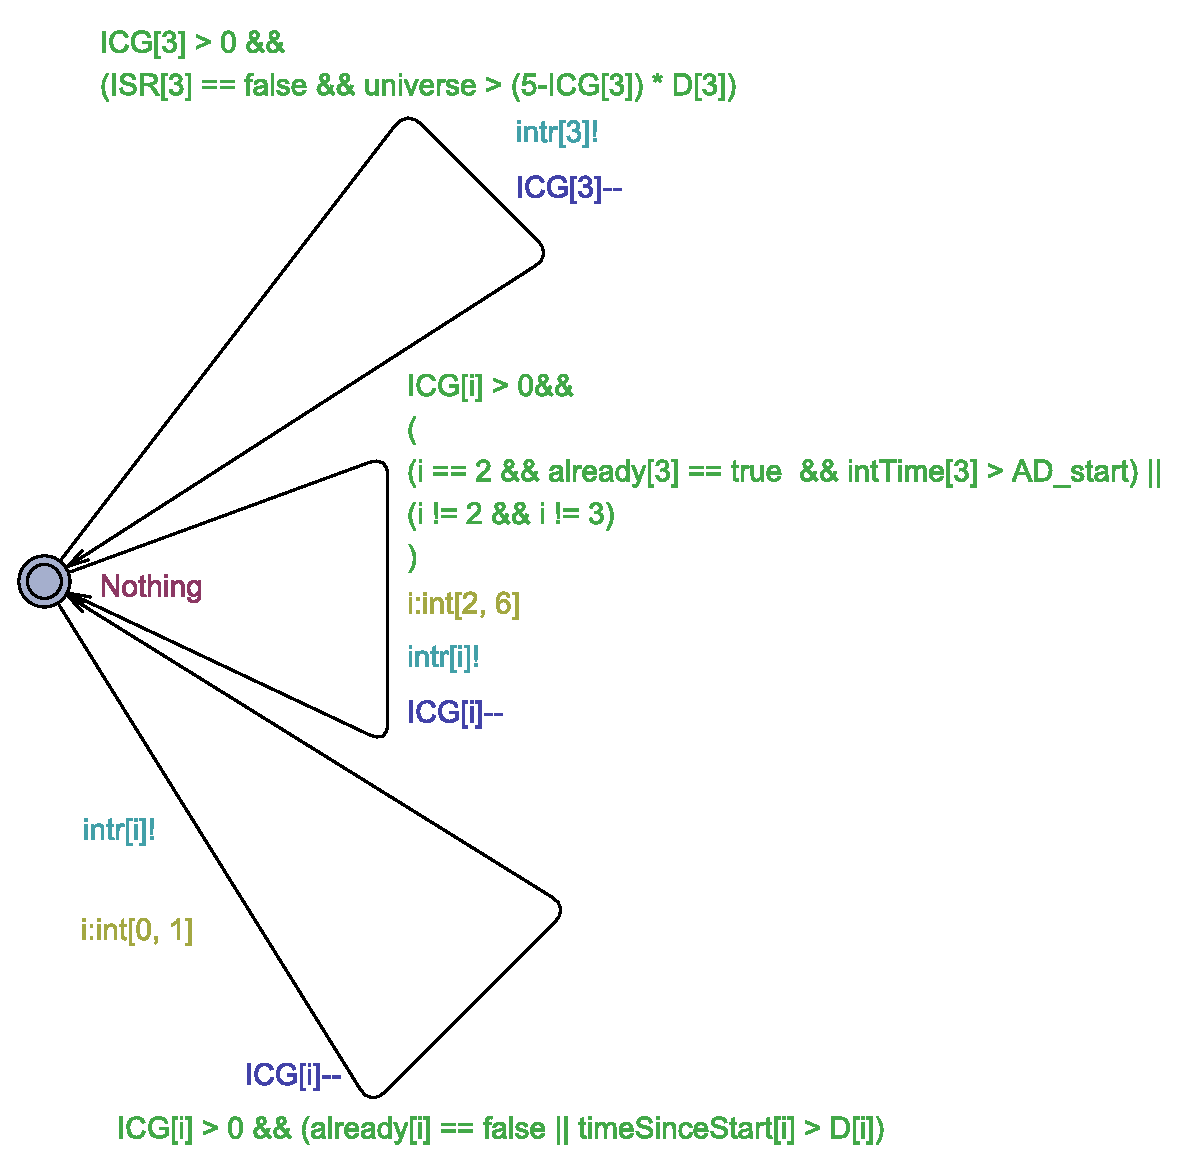
\includegraphics[width=0.9\textwidth]{env}
	\caption{某嵌入式平台中断模型:环境模板}
	\label{fig:exp_env}
\end{figure}

\subsection{系统声明}
\label{subsec:exp_model_decl}

系统声明很简单,如图~\ref{fig:exp_model_decl} 所示。在此不赘述。

\begin{figure}[H]
	\centering
	\begin{lstlisting}
	intr0 = Interrupt(0);
	intr1 = Interrupt(1);
	intr2 = AD(2);
	intr3 = Interrupt(3);
	intr4 = Interrupt(4);
	intr5 = Interrupt(5);
	intr6 = Interrupt(6);
	environment = env();
	system intr0, intr1, intr2, intr3, 
		intr4, intr5, intr6, environment
	\end{lstlisting}
	\caption{某嵌入式平台中断模型:系统声明}
	\label{fig:exp_model_decl}
\end{figure}

\section{分析与验证}
\label{sec:experiment}

在构建完模型之后,我们用\uppaal 提供的模拟器和验证对模型进行分析验证。首先,我们
对性质~\ref{property:all} 尝试验证。性质~\ref{property:all} 表示所有中断都不
会进入Error位置,即所有中断均不会超时。

\begin{property}
	A[] not (intr0.Error || intr1.Error || intr2.Error || intr3.Error 
	|| intr4.Error || intr5.Error || intr6.Error) 
	\label{property:all}
\end{property}

然而,该性质验证失败,反例如图~\ref{fig:exp_counter} 所示。我们跟随该反例复原
一下执行流程。首先3号中断触发,没有其他任何干扰因素,3号中断运行至结束。此时2号
中断,即AD中断触发条件满足,AD中断触发。AD中断执行到EOI指令之后,ISR对应位复位,
此时IRR和ISR所有为均为0,栈内只有AD中断。此时,4号中断触发,抢占CPU。此时,栈内
4号中断在AD中断之上,也就是说在4号中断执行结束之前,AD中断会被一直阻塞。由
\ref{subsec:exp_decl} 小节的定义可知$T_4=1011us$,$T^\prime_2=500us$,很显然,
$T_4>T^\prime_2$。因此,AD中断会超时。在与合作方工程师交流之后,我们一致认为在
系统这种中断触发序列是有可能的。避免方式也很简单,只要将4号中断的触发时机提前,
保证其在AD执行到EOI之前触发即可。

\begin{property}
	A[] not (intr0.Error || intr1.Error || intr3.Error || intr4.Error || 
	intr5.Error || intr6.Error) 
	\label{property:some}
\end{property}

接着我们尝试验证AD中断之外的其他中断的实时性。经过尝试,性质~\ref{property:some}
在消耗数小时后报告内存溢出,验证中止。这个结果在意料之中,因为在~\ref{subsec:exp_decl} 
小节的定义中,我们可以看到0号中断总共可以触发50次,这会极度增大状态空间,内存
溢出是正常。在尝试了各种办法之后,只有在将0号中断的数量修改到5以下,\uppaal 才会
给出验证结果\pozhehao 验证通过。

\begin{figure}[H]
	\centering
	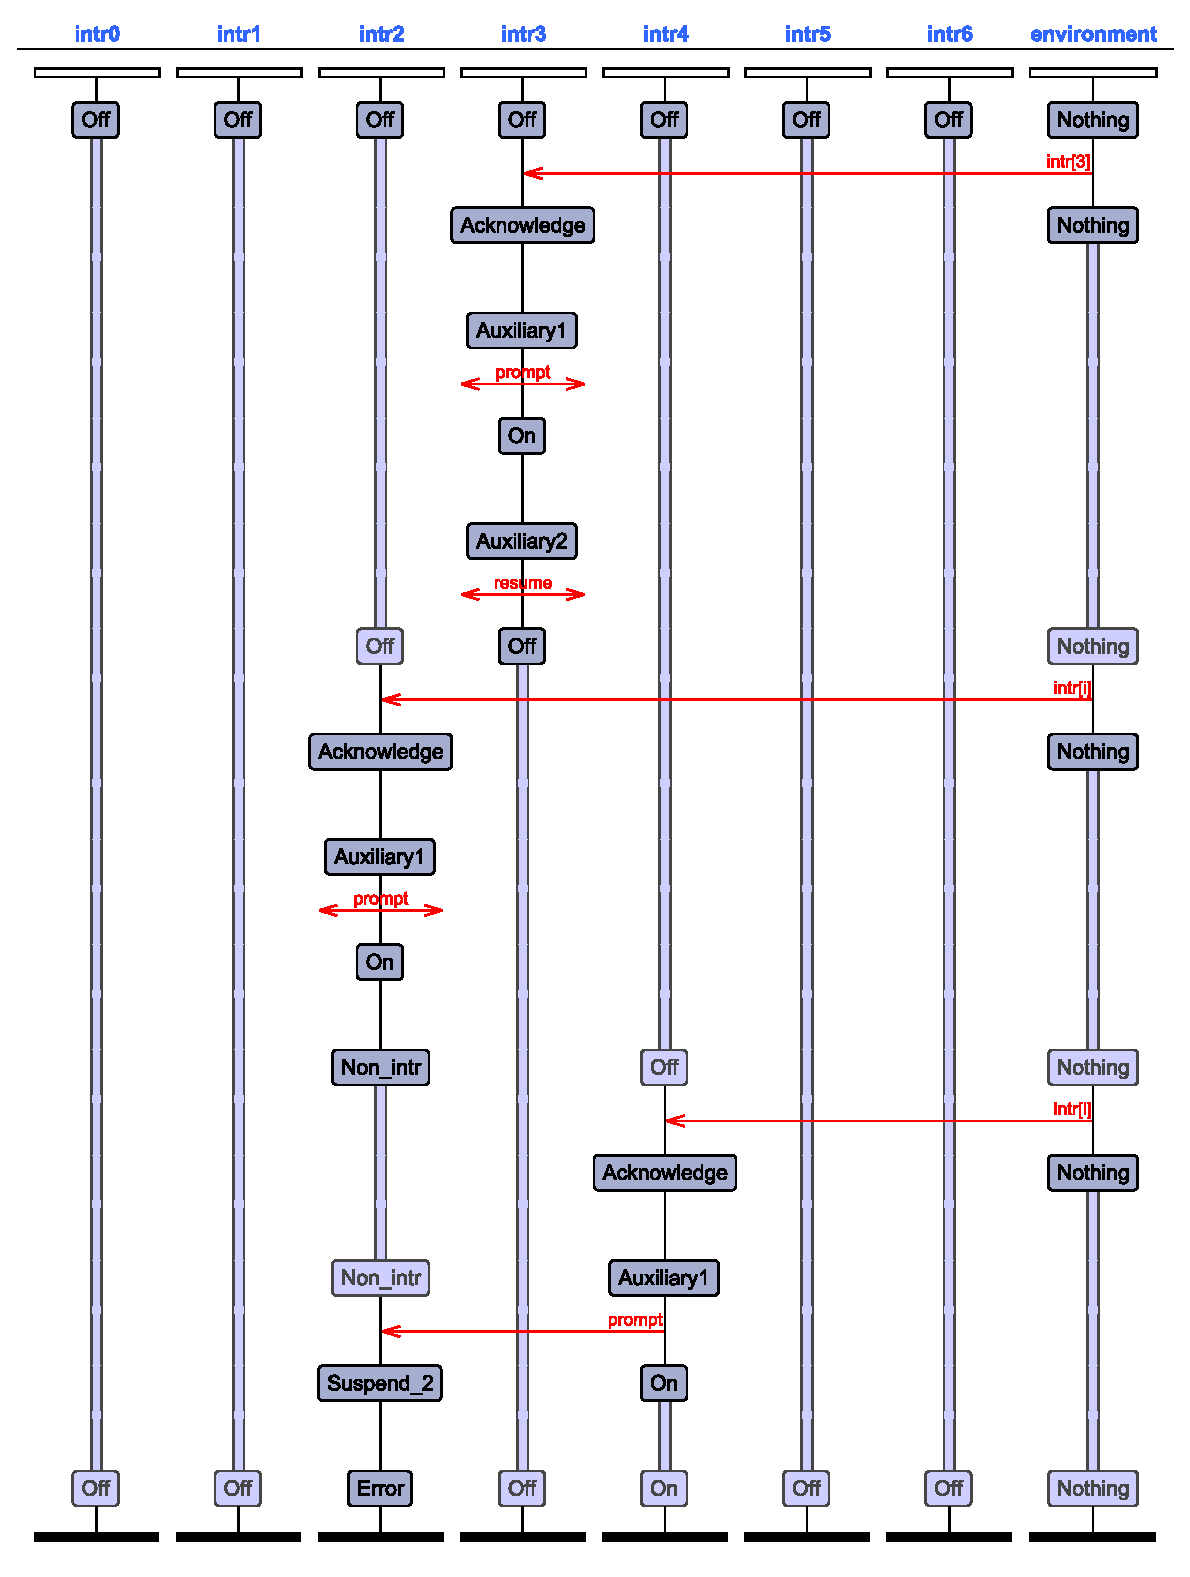
\includegraphics[width=\textwidth]{msc}
	\caption{性质~\ref{property:all} 的反例}
	\label{fig:exp_counter}
\end{figure}

\section{本章小结}
\label{sec:sum_4}

本章结合实际项目,对某嵌入式平台上的中断驱动程序进行分析,对其中断设置在\uppaal 中
构建了形式化模型,然后对其实时性属性进行分析和验证。该工作成功找出一个可能违反中
断实时性要求的反例,并与对方工程师交流得到确认。然而,由于状态空间太大,该模型对
其他中断的实时性是否满足要求并没有给出一个最终的结论。